\documentclass[preprint,12pt,a4paper]{elsarticle}

\usepackage{amssymb}
\usepackage{amsmath}
\usepackage{graphicx}
\usepackage{booktabs}
\usepackage{hyperref}
\usepackage{listings}
\usepackage{xcolor}
\usepackage{tikz}
\usepackage{multirow}
\usepackage{placeins}
\usepackage{array}
\usepackage{tabularx}
\usepackage{microtype}
\usetikzlibrary{arrows.meta,positioning,shapes.geometric,fit,backgrounds,calc}

% --- THORSTEN-18 TRACKING VERSION ---
%     Only the 18 supervisor comments (v21, May 2026) are highlighted.
%     All previous revision rounds are baked in as plain black text.
%     TEAL (\revt) = responses to Thorsten's 18 comments on the
%     final manuscript submitted to SoftwareX. ---
\definecolor{RevisionRed}{RGB}{180,0,0}
\definecolor{RevisionBlue}{RGB}{0,76,153}
\definecolor{RevisionGreen}{RGB}{0,120,60}
\definecolor{RevisionOrange}{RGB}{180,90,0}
\definecolor{RevisionViolet}{RGB}{120,0,180}
\definecolor{RevisionTeal}{RGB}{0,130,120}
\definecolor{RevisionMagenta}{RGB}{180,0,120}
% All previous revision rounds baked in (plain black) ---
% only the 18 Thorsten comments (\revt) are highlighted in teal.
\newcommand{\rev}[1]{{#1}}
\newcommand{\revb}[1]{{#1}}
\newcommand{\revg}[1]{{#1}}
\newcommand{\revo}[1]{{#1}}
\newcommand{\revr}[1]{{#1}}
\newcommand{\revn}[1]{{#1}}
\newcommand{\revt}[1]{{#1}}
\newcommand{\revv}[1]{{#1}}

\lstset{
  language=Python,
  basicstyle=\ttfamily\footnotesize,
  keywordstyle=\color{blue},
  commentstyle=\color{gray},
  stringstyle=\color{red!70!black},
  frame=single,
  breaklines=true,
  captionpos=b,
}

\emergencystretch=2em

\journal{SoftwareX}

\begin{document}

\begin{frontmatter}

\title{\texttt{weatherisk}: A Python Package for Spatial Clustering
  of Climate Extremes via Max-Stable Processes}

\author[awi,uni]{Widad Kchikach\corref{cor1}}
\ead{widad.kchikach@awi.de}
\cortext[cor1]{Corresponding author}

\author[uni]{Thorsten Dickhaus}
\author[awi,uni]{Gerrit Lohmann}

\address[awi]{Alfred Wegener Institute Helmholtz Centre for Polar
  and Marine Research, Bremerhaven, Germany}
\address[uni]{University of Bremen, Bremen, Germany}

\begin{abstract}
We present \texttt{weatherisk}, an open-source Python package for
identifying regions of homogeneous extremal dependence in gridded
climate-model output. The package implements a
complete analysis pipeline: \revt{seasonal-trend decomposition} removes
long-term trends from raw monthly fields; annual block maxima are
extracted and fitted with \revt{generalised extreme-value}
distributions; marginals are transformed to unit Fr\'{e}chet
scale---the standard heavy-tailed reference form required by max-stable
models---and local spatial-dependence parameters are estimated before
grid cells are partitioned into coherent regions. Two clustering
schemes are supported, Local Estimates Clustering and Extremal
Dependence Clustering. The test suite compares each pipeline stage
with stored outputs of the original R implementation, so R is not
needed to install, run or test the package. We demonstrate \texttt{weatherisk} on a global-precipitation
case study using the \revt{Alfred Wegener Institute (AWI)}-ESM-1-1-LR model \revn{(T63 grid, $192\times96$
cells, 1850--2005),} executed on the AWI \emph{albedo} high-performance cluster, \revn{revisiting a published clustering study
and obtaining a spatially consistent result in Python. The outcome}
is a reproducible, scalable framework for
spatial-extremes analysis, suited equally to synthetic benchmarks and
publication-scale climate-model output.
\end{abstract}

\begin{keyword}
\revt{spatial extremes \sep max-stable process \sep extremal dependence \sep spatial clustering \sep Python}
\end{keyword}
% C1: keywords reordered — science-first (broad domain → method → concept → application → tool); SoftwareX imposes no ordering rule

\end{frontmatter}

%% ============================================================
\section*{Metadata}
\label{sec:metadata}
%% ============================================================

Table~\ref{tab:metadata} summarises the mandatory software metadata
for the current release of \texttt{weatherisk}.

\begin{table}[!h]
\small
\begin{tabularx}{\textwidth}{|l|>{\raggedright\arraybackslash}p{4.9cm}|>{\raggedright\arraybackslash}X|}
\hline
\textbf{Nr.} & \textbf{Code metadata description} & \textbf{Metadata} \\
\hline
C1 & Current code version & \revn{v0.1.1} \\ % TODO: bump to v0.1.2 at release
\hline
C2 & Permanent link to code/repository &
  \url{https://github.com/wkchikach99-byte/weatherisk} \\
\hline
C3 & Permanent link to Reproducible Capsule &
  \revn{\url{https://doi.org/10.5281/zenodo.20108563}} \\ % TODO: new Zenodo DOI for v0.1.2
\hline
C4 & Legal Code License & MIT \\
\hline
C5 & Code versioning system used & git \\
\hline
C6 & Software code languages, tools, and services used &
  Python~3.10+; SLURM (optional, for HPC runs) \\
\hline
C7 & Compilation requirements, operating environments
  \& dependencies &
  Python~$\geq$3.10; NumPy; SciPy; pandas; matplotlib;
  Click; xarray; netCDF4; scikit-learn; Cartopy; h5py;
  statsmodels. Optional for development: pytest, pytest-cov, ruff,
  mypy, pyreadr, psutil. R is not required. The validation fixtures
  were generated once with the reference R implementation and ship
  with the repository as frozen CSV and binary files. \\
\hline
C8 & Link to developer documentation &
  \url{https://github.com/wkchikach99-byte/weatherisk} \\
\hline
C9 & Support email for questions & widad.kchikach@awi.de \\
\hline
\end{tabularx}
\caption{Code metadata (mandatory).}
\label{tab:metadata}
\end{table}


%% ============================================================
\section{Motivation and significance}
\label{sec:motivation}
%% ============================================================

Extreme weather events such as heavy precipitation or heat waves
rarely act on a single location; they typically unfold across broad
regions at once~\cite{davison2012}. Understanding \emph{where} such events tend to
co-occur matters enormously for regional risk assessment, reinsurance,
and infrastructure planning. Ignoring the spatial footprint of
extremes can lead to a serious underestimate of aggregate losses.

\revg{While mean climate trends carry important information,
socioeconomic impacts are driven disproportionately by extreme events
rather than by shifts in average conditions~\cite{davison2012}. Infrastructure
failures, crop losses, and flood damage are governed by tail
probabilities (the chances of exceeding a rarely reached, very high
threshold)---not by means---of precipitation and temperature
distributions. Getting the tail behaviour and its spatial dependence
structure right is therefore central to any serious risk
quantification.}

\revg{Extremes also behave differently from everyday climate
variability: they show non-Gaussian distributions, heavy
tails (where extreme values occur far more often than a bell-curve
distribution would predict), and \revt{extremal dependence---the
tendency for extreme events at different locations to co-occur}%
---none of which standard
covariance-based techniques adequately represent~\cite{dehaan2006}. Extreme
value theory (EVT) provides the rigorous mathematical framework
for this regime. \revt{One standard approach in EVT is the
\emph{block maxima method}: the block maximum is the single largest
observed value within a fixed time window---here, one calendar year.
Under certain conditions, the distribution
of annual block maxima can be approximated well by a
\emph{generalised extreme-value} (GEV) distribution, a
three-parameter family~\cite{dehaan2006,padoan2010}. The family of GEV distributions contains the limiting
distribution of block-wise maxima for a broad range of
data-generating distributions.} Capturing the
spatial dependence structure of these extremes across many grid
cells requires both a statistically sound framework and software
that can handle the associated computational burden---the dual
motivation for the present work.}


\emph{Max-stable processes} are the standard framework for
modelling joint tail behaviour across space~\cite{dehaan2006,padoan2010}.
Following Contzen et al.~\cite{contzen2025}, fitting these models at each location
yields anisotropy parameters that capture the strength and
directional orientation of local spatial dependence.
Grid cells with similar parameter estimates can then be grouped
into \emph{clusters}---geographically connected regions in which
the extremal dependence structure is approximately uniform.

An R-based pipeline that implements this workflow was developed
by Contzen et al.~\cite{contzen2025}. It \revt{fits max-stable processes to given
climate datasets},
estimates local anisotropy parameters via pairwise composite
likelihood~\cite{padoan2010} \revr{(see Section~\ref{sec:architecture} for the
technical details)}, computes a pairwise dissimilarity score between
all grid cells based on the geometric overlap of their fitted
anisotropy ellipses, and \revt{groups} cells by hierarchical clustering. \revt{Up
to now, however, the existing} implementation is fragmented across independent
R scripts tied together by SLURM shell files\revt{. That implementation
served its intended purpose very well: it provided the empirical
illustration needed for the statistical methodology paper by Contzen
et al.~\cite{contzen2025}. As the method gains wider adoption and is applied to
larger or more varied datasets, however, a structured and installable
package becomes necessary, and that is precisely the gap
\texttt{weatherisk} fills.}
\rev{This limitation becomes particularly acute in climate-model
applications, where extremes are, by definition, rare, and stable
statistical inference requires long time series---decades or
centuries. Modern coupled models such as AWI-ESM-1-1-LR produce
monthly output on global grids (e.g.\ T63, $192 \times 96 = 18{,}432$ cells) spanning hundreds of simulated years.  Processing
these heavy NetCDF archives before any clustering can begin involves
detrending, block-maxima extraction, GEV marginal fitting (estimating
a separate GEV distribution independently at each grid cell), and
Fr\'{e}chet transformation at every grid cell.  Scientific software
for this problem therefore has to do more than implement the
mathematics: it must also provide a reproducible preprocessing chain,
checkpoint/restart support for long-running jobs, and numerically
efficient kernels that scale from laptops to high-performance
computing facilities.}

\texttt{weatherisk} solves this problem by re-implementing the full
pipeline in a single Python package that can be installed with
\texttt{pip install}.  It is an independent implementation of the
method of Contzen et al.~\cite{contzen2025}, tested stage by stage
against stored outputs of the original R code on reduced inputs, and
it adds several practical features:
\begin{itemize}
\item \rev{a complete preprocessing chain for climate-model output:
  STL (Seasonal-Trend decomposition using Loess) detrending, annual
  block-maxima extraction, GEV fitting, and Fr\'{e}chet transformation
  (a probability-integral step that maps each grid cell's fitted GEV
  values to a common unit-Fr\'{e}chet scale required by the max-stable
  model)};
\item \rev{checkpoint/restart support and scalable execution
  strategies for heavy CMIP6\revo{ (Coupled Model Intercomparison
  Project Phase~6)}-style workloads on high-performance
  computing (HPC) infrastructure}; and
\item \rev{a 196-test validation suite, including 30~end-to-end % TODO(U4): regenerate from test inventory
  CMIP6 parity tests (Section~\ref{sec:validation})}.
\end{itemize}

\rev{To demonstrate the software on a publication-level workload, we
include a \revb{Python-based revisit of the Figure~9 case study} from Contzen et al.~\cite{contzen2025} on the
AWI-ESM-1-1-LR historical precipitation dataset and provide a
systematic validation analysis (Section~\ref{sec:validation}) that
states, for each pipeline stage, the criterion used to compare it with
the original R implementation.}

Existing Python packages do support parts of the extreme-value workflow.
For example, \texttt{pyextremes}~\cite{pyextremes} and
\texttt{scikit-extremes}\footnote{\url{https://github.com/kikocorreoso/scikit-extremes}}
focus on univariate extreme-value analysis, while the R package
\texttt{SpatialExtremes}~\cite{spatialextremes} provides max-stable simulation.
However, to our knowledge, no existing Python package offers the
integrated spatial-extremes workflow implemented here: max-stable
simulation, local composite-likelihood estimation, and ellipse-based
spatial clustering of extremes in one package.

%% ============================================================
\section{Software description}
\label{sec:description}
%% ============================================================

\subsection{Software architecture}
\label{sec:architecture}

\texttt{weatherisk} is a pip-installable Python package organised
into 18~modules and a CLI entry point.  Figure~\ref{fig:workflow} % TODO: git ls-files lists 21 modules plus cli.py (excluding __init__.py); recount at the v0.1.2 tag
shows the overall workflow.

\rev{The processing pipeline consists of seven stages. The first
stage contains three sub-steps that together convert raw climate-model
output into the standardised representation required by the
subsequent statistical analysis:}

\begin{enumerate}
\item \textbf{\rev{Preprocessing.}}
  \begin{enumerate}
  \item[\textbf{(a)}] \textbf{\rev{STL decomposition (detrending).}}
    \rev{Raw monthly precipitation fields are decomposed using the
    STL method of Cleveland et al.~\cite{cleveland1990}, using the
    \texttt{statsmodels} implementation with a 12-month period,
    robust fitting, a constant (degree-0) seasonal smoother and a
    seasonal window at least as long as the series.
    These settings correspond to the R call \texttt{stl(s.window =
    "periodic", robust = TRUE)} in the reference workflow.  The trend component is
    subtracted, retaining the seasonal cycle and residuals. \revt{This
    step removes the long-term trend from the series,
    leaving the seasonal cycle and interannual residuals available for
    extreme-value analysis.}}
  \item[\textbf{(b)}] \textbf{\rev{Annual block-maxima extraction.}}
    \rev{From the detrended monthly series, the annual maximum
    precipitation value is extracted for each grid cell, \revt{keeping
    only years for which observations are available in all 12 months}.
    The result is an
    $(n_{\text{years}} \times n_{\text{cells}})$ matrix of annual
    extremes that feeds the marginal fitting step. \revt{Taking the
    annual maximum thereby instantiates} the \revt{block maxima}
    approach of classical EVT~\cite{dehaan2006}.}
  \item[\textbf{(c)}] \textbf{\rev{GEV fitting and Fr\'{e}chet
    transformation.}}
    \rev{A GEV distribution is fitted independently at each grid cell
    by maximum likelihood. Before fitting, cells that are entirely
    missing or have near-zero variance are excluded; isolated missing
    values in the remaining cells are replaced by the cell-wise mean.
    Any cell that still yields non-finite GEV or Fr\'{e}chet values
    after fitting is dropped. In the full AWI-ESM-1-1-LR run, all
    $192 \times 96 = 18{,}432$ cells passed this screen. The fitted
    GEV at each cell is then used to apply the probability integral
    transform: each annual maximum is mapped through its own GEV
    cumulative distribution function, producing a value on the
    unit Fr\'{e}chet scale (the common marginal form required by
    max-stable models, as described in Section~\ref{sec:motivation}).
    \revr{This puts all cells on an equal footing before spatial
    dependence is estimated: what remains captures where extremes
    co-occur, not how large they are at any individual site.}
    Values are clipped to $[0.05,\, n_{\text{years}}^{2}]$ to
    suppress numerical artefacts at the tails.}
  \end{enumerate}
\item \textbf{Simulation} (for validation on synthetic data).
  Synthetic max-stable random fields with
  user-specified spatially varying anisotropy are generated on a
  regular grid following the spectral construction of
  Schlather~\cite{schlather2002}. These fields serve as controlled test cases whose
  true parameters are known by construction.
\item \textbf{Local estimation.}
  For each grid cell, we estimate the three local anisotropy
  parameters---semi-axis lengths $a$ and $b$ (controlling the range
  and degree of directional asymmetry of spatial dependence) and a
  rotation angle $\gamma$ (the principal direction of dependence)---by
  maximising a pairwise composite likelihood~\cite{padoan2010,contzen2025}\revr{, which sums
  log-likelihood contributions over neighbouring grid-cell pairs;
  this avoids fitting the full joint spatial distribution at once and
  makes estimation computationally feasible on large grids.} The
  optimisation runs over all neighbouring pairs within grid-point
  distance $\varepsilon$ (default $\varepsilon=5$).
  \rev{Neighbours are enumerated in a fixed stencil order
  (x-offset varies fastest) matching the R reference, and at least
  three valid neighbours are required; cells with fewer than five
  valid pairs receive default estimates $(a,b,\gamma) = (1,0,0)$.
  The likelihood is maximised with the bounded quasi-Newton method
  L-BFGS-B from SciPy, started from five Latin-hypercube points % TODO(U3): start budget set by the U3 sweep
  (seed = 42) to reduce sensitivity to local optima~\cite{contzen2025}.
  In the CMIP6 pipeline, Fr\'{e}chet values are rounded to 11 decimal
  places before optimisation. The stored R reference inputs have a
  fixed decimal precision, and the rounding keeps last-bit differences
  from moving the optimiser to a different optimum of equal likelihood.}
\item \textbf{\rev{Spatial smoothing.}}
  \rev{The raw estimates $(a_i, b_i, \gamma_i)$ \revt{(where
  subscript $i$ indexes the grid cell)} are smoothed by a
  moving average over grid cells within a smoothing radius (default
  2.0 in grid-point units).  Angular wrapping is applied to the
  rotation angle $\gamma$ to account for its directional
  periodicity ($+90^{\circ} \equiv -90^{\circ}$).}
\item \textbf{Clustering.}
  From the smoothed parameter estimates, we assemble a pairwise
  dissimilarity matrix and apply average-linkage hierarchical
  agglomerative clustering~\cite{contzen2025} to group grid cells into regions.
  The number of clusters $k$ is set automatically, following Contzen
  et al.~\cite{contzen2025}. The threshold is a quantile of all
  pairwise dissimilarities (default: 30\textsuperscript{th}
  percentile), and $k$ is the number of dendrogram merge heights
  that exceed it.
  Two dissimilarity measures are available:
  \begin{itemize}
  \item \textbf{LEC} (Local Estimates Clustering~\cite{contzen2025}; ellipse-overlap
    dissimilarity $D_2$): Jaccard-like overlap of the anisotropy
    ellipses\revo{ (a ratio of intersection to union area, ranging
    from 0 for non-overlapping to 1 for identical ellipses; here
    used as a geometrically interpretable dissimilarity $1 - \text{overlap}$)}.
    \revr{Each grid cell's fitted parameters $(a, b, \gamma)$ define
    an ellipse in 2D space. Two cells whose ellipses overlap strongly
    have a similar dependence geometry, so high overlap means low
    dissimilarity. The ratio $D_2$ was introduced by Contzen
    et al.~\cite{contzen2025} as a geometrically clear way to measure this.}
  \item \textbf{EDC} (Extremal Dependence Clustering~\cite{contzen2025}; madogram-based
    dissimilarity $D_1$, following Cooley et al.~\cite{cooley2006} and Saunders et al.~\cite{saunders2021}):
    \revo{The madogram is a rank-based summary of extremal
    dependence: computed from order statistics without parametric
    assumptions, it maps onto pairwise extremal coefficients that
    range from 1 (complete dependence: extreme events at the two
    sites always co-occur) to 2 (independence), with intermediate
    values reflecting partial co-occurrence~\cite{cooley2006}.  Contzen et al.~\cite{contzen2025}
    adopt this approach alongside the ellipse method, providing an
    alternative non-parametric dissimilarity $D_1$ for
    dependence-based regionalisation.}
  \end{itemize}
\item \textbf{\rev{In-cluster re-estimation.}}
  \rev{Within each cluster, the dependence parameters are
  re-estimated using all data from the cluster's grid cells via
  global pairwise composite-likelihood maximum-likelihood estimation
  (MLE; distance cutoff: $4.0
  \times$ neighbour radius, 3 restarts per cluster). The
  goodness-of-fit of each method is assessed.}
\end{enumerate}

\begin{figure}[ht]
\centering
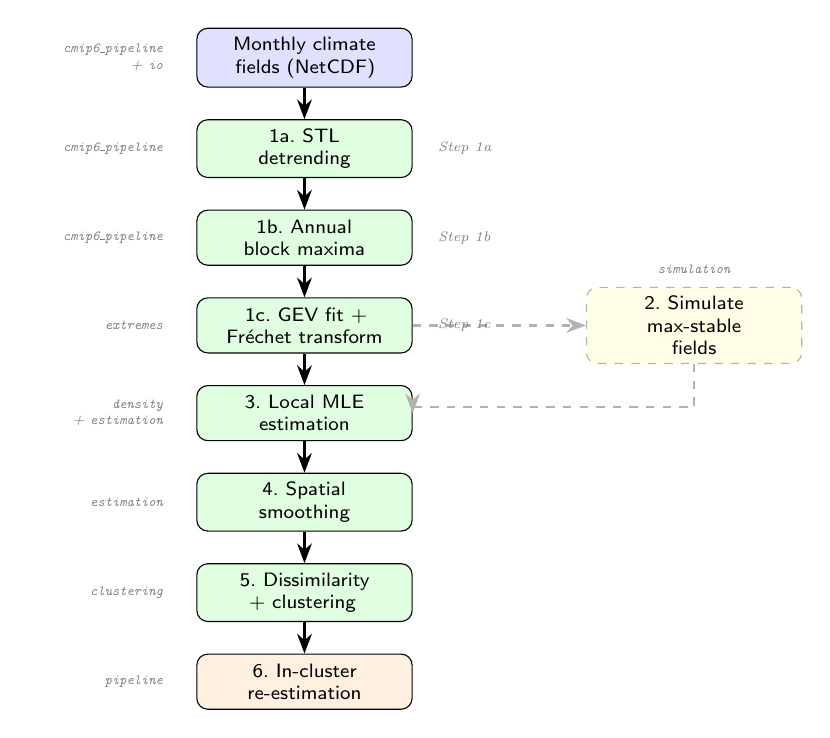
\begin{tikzpicture}[
  box/.style={draw, rounded corners=4pt, minimum width=2.6cm,
    minimum height=0.7cm, font=\sffamily\scriptsize,
    align=center, text width=2.5cm},
  data/.style={box, fill=blue!12},
  proc/.style={box, fill=green!12},
  outbox/.style={box, fill=orange!12},
  simbox/.style={box, fill=yellow!10, draw=gray!60, dashed},
  arr/.style={-{Stealth[length=2.5mm]}, thick},
  arrdashed/.style={-{Stealth[length=2.5mm]}, thick, dashed, gray!60},
  note/.style={font=\itshape\tiny, text=gray},
  node distance=0.4cm,
]

\node[data] (raw) {Monthly climate\\fields (NetCDF)};

\node[proc, below=of raw] (stl)
  {\rev{1a.\ STL\\detrending}};
\node[proc, below=of stl] (bm)
  {\rev{1b.\ Annual\\block maxima}};
\node[proc, below=of bm] (frech)
  {\rev{1c.\ GEV fit +\\Fr\'{e}chet transform}};
\node[proc, below=of frech] (mle)
  {3.\ Local MLE\\estimation};
\node[proc, below=of mle] (smooth)
  {4.\ Spatial\\smoothing};
\node[proc, below=of smooth] (clust)
  {5.\ Dissimilarity\\+ clustering};
\node[outbox, below=of clust] (out)
  {6.\ In-cluster\\re-estimation};

\draw[arr] (raw) -- (stl);
\draw[arr] (stl) -- (bm);
\draw[arr] (bm) -- (frech);
\draw[arr] (frech) -- (mle);
\draw[arr] (mle) -- (smooth);
\draw[arr] (smooth) -- (clust);
\draw[arr] (clust) -- (out);

% Stage 2: simulation side-branch (optional validation path)
\node[simbox, right=2.2cm of frech] (sim)
  {\revt{2.\ Simulate\\max-stable\\fields}};
\node[note, above=0.05cm of sim, text width=2.5cm, align=center]
  {\texttt{simulation}};
\draw[arrdashed] (frech.east) -- (sim.west);
\draw[arrdashed] (sim.south) -- ++(0,-0.55) -| (mle.east);

% Module names on the left
\node[note, left=0.3cm of raw, text width=1.6cm, align=right]
  {\texttt{cmip6\_pipeline}\\+ \texttt{io}};
\node[note, left=0.3cm of stl, text width=1.6cm, align=right]
  {\rev{\texttt{cmip6\_pipeline}}};
\node[note, left=0.3cm of bm, text width=1.6cm, align=right]
  {\rev{\texttt{cmip6\_pipeline}}};
\node[note, left=0.3cm of frech, text width=1.6cm, align=right]
  {\texttt{extremes}};
\node[note, left=0.3cm of mle, text width=1.6cm, align=right]
  {\texttt{density}\\+ \texttt{estimation}};
\node[note, left=0.3cm of smooth, text width=1.6cm, align=right]
  {\texttt{estimation}};
\node[note, left=0.3cm of clust, text width=1.6cm, align=right]
  {\texttt{clustering}};
\node[note, left=0.3cm of out, text width=1.6cm, align=right]
  {\texttt{pipeline}};

% Stage labels on the right
\node[note, right=0.2cm of stl] {Step 1a};
\node[note, right=0.2cm of bm] {Step 1b};
\node[note, right=0.2cm of frech] {Step 1c};

\end{tikzpicture}
\caption{\rev{Processing pipeline of \texttt{weatherisk}. Stage~1
  (a--c) is the preprocessing chain added for climate-model data;
  stages~3--6 implement the core statistical methodology of Contzen
  et al.~\cite{contzen2025}. Module names are shown on the left.\revt{ Stage~2
  (dashed box, right): \texttt{simulation.py} generates simulated
  max-stable fields on a regular 2-D grid with user-chosen dependence
  parameters (Schlather~\cite{schlather2002} spectral construction) and passes them to
  Stage~3 to check whether the pipeline gives back those known
  values.}}}
\label{fig:workflow}
\end{figure}

\subsection{Software functionalities}
\label{sec:functionalities}

Section~\ref{sec:architecture} describes the end-to-end workflow.
This subsection instead summarises the main software components and
their roles within the package.

\paragraph{Covariance modelling (\texttt{covariance})}
This module implements the anisotropic covariance functions used by
the max-stable dependence model, including stationary and
non-stationary formulations and the conversion between covariance and
extremal-coefficient representations.

\paragraph{Simulation (\texttt{simulation})}
The simulation module generates synthetic max-stable fields with
spatially varying anisotropy. These synthetic datasets are used for
method development, controlled validation experiments, and regression
tests against known parameter fields.

\paragraph{Preprocessing and extremes (\texttt{cmip6\_pipeline}, \texttt{netcdf}, \texttt{extremes})}
These components handle gridded climate-model input, including NetCDF
loading, STL detrending of monthly series, annual block-maxima
extraction, GEV fitting, and transformation to unit Fr\'{e}chet
margins. Together they provide the climate-data preprocessing chain
required before spatial dependence can be estimated.

\paragraph{Estimation (\texttt{density}, \texttt{estimation})}
These modules implement pairwise composite-likelihood estimation of
the local anisotropy parameters $(a,b,\gamma)$, the subsequent spatial
smoothing step, and the in-cluster re-estimation routines used after
clustering. They also contain the numerical safeguards needed for
stable optimisation on large grids.

\paragraph{Clustering (\texttt{clustering})}
This module provides the two regionalisation methods implemented in
\texttt{weatherisk}: LEC (Local Estimates Clustering), based on
ellipse-overlap dissimilarity, and EDC (Extremal Dependence
Clustering), based on madogram-derived extremal dependence. It also provides
the hierarchical clustering utilities that convert these
dissimilarities into region labels.

\paragraph{Scalability and execution (\texttt{scalable}, \texttt{cli})}
These components support large production runs through parallel
execution, checkpoint/restart handling, and command-line entry points
for the main workflows. They are designed to make the same code base
usable both for local experiments and for HPC-scale Figure~9
\revb{case-study analysis}.

\paragraph{Plotting and outputs (\texttt{plotting}, \texttt{map\_plotting})}
The plotting modules generate diagnostic figures, synthetic-study
visualisations, and the publication-style cluster maps used in the CPC
and CMIP6 workflows. They provide the final user-facing outputs of the
pipeline in addition to the saved numerical arrays.

\subsection{Computational performance}
\label{sec:performance}

The dominant costs are the $O(n^2)$ pairwise dissimilarity matrix and
per-cell local MLE optimisation.
\texttt{weatherisk} reduces both in four ways:

\begin{enumerate}
\item \textbf{Batch covariance.}
  All $n^2$ entries are evaluated in a single vectorised NumPy call;
  $2\times 2$ matrix inverses use the analytic closed-form formula.

\item \textbf{Pre-drawn ellipse overlap (LEC).}
  Each fitted ellipse is rasterised once; pairwise overlap areas
  are computed with bitwise operations over batches of 256 pairs.

\item \textbf{Fast pairwise distance (EDC).}
  \texttt{scipy.spatial.distance.\allowbreak{}cdist} evaluates all
  pairwise rank-based distances in a single compiled-C call.

\item \textbf{Parallel local estimation.}
  Per-cell MLE tasks are distributed via Python's
  \texttt{multiprocessing}; shared data is loaded once per worker.
\end{enumerate}

On a 6$\times$6 synthetic input, the Python pipeline % TODO(U6): pure-Python rerun (timing measured before v0.1.2)
completed in 17.9\,s compared with 43.9\,s for the original
R~implementation---a 2.5$\times$ speed-up on an identical workload.
The full AWI-ESM-1-1-LR T63 grid (18{,}432 cells, 156~years) was
run on the \revt{Alfred Wegener Institute (AWI)} \emph{albedo} HPC cluster using 16~parallel workers,
completing in approximately 4~hours with peak memory below 2\,GiB; % TODO(U6): pure-Python rerun
SLURM scripts and setup are provided under \texttt{hpc/}.


\paragraph{Command-line interface (\texttt{cli})}
A single entry point exposes the main pipeline flows:
\begin{lstlisting}[numbers=none]
$ weatherisk validate --params stripes \
    --resolution 10 --n-sim 20 --seed 42
$ weatherisk maps --variable precip
\end{lstlisting}

%% ============================================================
\section{Illustrative examples}
\label{sec:examples}
%% ============================================================

We demonstrate \texttt{weatherisk} with \rev{two} examples: one on
synthetic data \rev{and one \revb{Python-based revisit of Figure~9 from Contzen}
et al.~\cite{contzen2025} on the AWI-ESM-1-1-LR climate model}.

\subsection{Example~1: Synthetic validation}
\label{sec:ex-synthetic}

In this example, we simulate max-stable data on a 51$\times$51 grid
where the semi-major axis $b$ increases linearly from left to right,
creating vertical ``stripe'' regions.  The pipeline should recover
these stripes from the simulated data alone.

\begin{lstlisting}[caption={Running the stripes validation.},
  label=lst:validate]
from weatherisk.pipeline import run_nonstationary_pipeline

# Preset "paper_stripes": 51x51 grid on [-5,5]^2, 250 replicates,
# true semi-major axis b(x, y) = (x + 5)/2
result = run_nonstationary_pipeline(
    "paper_stripes", seed=42, n_workers=8,
)
print(result["k_edc"], result["k_lec"])
\end{lstlisting}

\noindent Listing~\ref{lst:app-validate} in \ref{app:code} runs the same
steps one function at a time.

Figure~\ref{fig:stripes} shows the result.  Panel~(a) displays the
EDC clusters ($k_{\text{edc}} = 7$), panel~(b) the LEC clusters % TODO(U6): pure-Python rerun; k values and the description below
($k_{\text{lec}} = 5$), and panel~(c) the true parameter field.
The true semi-major axis~$b$ increases smoothly from left to right
(panel~c), producing a continuous gradient from dark blue ($b
\approx 0$) on the left to light shading ($b \approx 5$) on the
right.  The EDC method (panel~a) uses seven clusters and captures
the overall left-to-right trend, but its boundaries are irregular:
some clusters extend horizontally across the domain, and the
transitions between adjacent regions do not follow the vertical
orientation of the true gradient.  The LEC method (panel~b), by
contrast, uses only five clusters yet produces boundaries that are
predominantly vertical, closely tracking the true transitions in
the parameter field.  The estimated within-cluster~$b$ values in
the LEC map also progress monotonically from dark to light,
mirroring the ground truth more faithfully than the EDC partition.
This controlled experiment illustrates that the Python
implementation recovers the known spatial structure,
consistent with the methodology of Contzen et al.~\cite{contzen2025}.
Section~\ref{sec:validation} describes how each stage is compared
with the original R code.

\begin{figure}[!htbp]
\centering
\includegraphics[width=0.95\textwidth]{figures/fig3_regenerated.png} % TODO(U6): replace with the pure-Python run
\caption{Synthetic validation on the ``stripes'' preset
  ($k_{\text{edc}} = 7$, $k_{\text{lec}} = 5$). % TODO(U6): pure-Python rerun
  (a)~EDC clusters coloured by estimated semi-major axis~$b$;
  (b)~LEC clusters coloured by estimated~$b$;
  (c)~true parameter field showing a smooth left-to-right
  gradient in~$b$ from 0 to~5.
  The LEC method recovers sharper, vertically aligned boundaries
  that closely match the ground truth, while the EDC method
  produces more irregular, horizontally extended partitions.}
\label{fig:stripes}
\end{figure}

\FloatBarrier

\rev{\subsection{Example~2: \revb{Revisiting the Figure~9 case study} --- AWI-ESM-1-1-LR
  global precipitation}}
\label{sec:ex-fig9}

\rev{To demonstrate the software on the same data used in the original
publication, we \revb{revisit the Figure~9 analysis} of Contzen et al.~\cite{contzen2025}.  The
experiment uses monthly precipitation from the AWI-ESM-1-1-LR
historical simulation (T63 grid, $192 \times 96$ cells, r1i1p1f1,
years 1850--2005) with the parameter settings listed in
Table~\ref{tab:fig9-params}, following Section~5 of~\cite{contzen2025}:}

\begin{table}[ht]
\centering
\begin{tabular}{ll}
\toprule
\textbf{Parameter} & \textbf{Value} \\
\midrule
Degrees of freedom $\nu$ & 5 \\
Covariance exponent $\alpha$ & 1 \\
Neighbour radius $\varepsilon$ & 5 (grid-point units) \\
Clustering quantile threshold & 30\textsuperscript{th} percentile \\
Model / experiment & AWI-ESM-1-1-LR / historical \\
Grid / resolution & T63 ($192 \times 96$) \\
Period & 1850--2005 (156~years) \\
\bottomrule
\end{tabular}
\caption{Parameter settings used for the Figure~9 \revb{case-study analysis},
  following Section~5 of Contzen et al.~\cite{contzen2025}. \revo{The degrees of
  freedom $\nu$ and covariance exponent $\alpha$ are parameters of
  the Schlather max-stable dependence model~\cite{schlather2002}: $\nu$ controls
  how quickly dependence decays with distance (higher $\nu$ gives
  weaker long-range dependence), and $\alpha \in (0,\,2]$
  controls the smoothness of the simulated fields.}}
\label{tab:fig9-params}
\end{table}

\rev{The full seven-stage pipeline (Section~\ref{sec:architecture}) was
executed on the AWI \emph{albedo} HPC cluster (16~CPU cores;
SLURM scripts in \texttt{hpc/}). The command-line invocation is:}

\begin{lstlisting}[caption={\revb{Running the Figure~9 case study on HPC}.},
  label=lst:fig9, numbers=none]
$ python scripts/reproduce_fig9.py \
    --data-dir /path/to/AWI-ESM-1-1-LR/pr/ \
    --workers 16  --output-dir output/cmip6_fig9 \
    --dpi 300
\end{lstlisting}

\rev{Figure~\ref{fig:fig9} shows the result, and
Table~\ref{tab:fig9-counts} compares the resulting cluster counts with
those reported by Contzen et al.~\cite{contzen2025}:}

\begin{table}[ht]
\centering
\begin{tabular}{lcc}
\toprule
\textbf{Method} & \textbf{Contzen et al.~\cite{contzen2025}} &
  \textbf{\texttt{weatherisk}} \\
\midrule
EDC ($k_{\text{edc}}$) & 104 & 142 \\ % TODO(U6): pure-Python rerun
LEC ($k_{\text{lec}}$) & 24 & 21 \\ % TODO(U6): pure-Python rerun
\bottomrule
\end{tabular}
\caption{Cluster counts reported in Contzen et al.~\cite{contzen2025} and obtained
  with \texttt{weatherisk} for the full Figure~9 \revb{case-study run}.}
\label{tab:fig9-counts}
\end{table}

\rev{The LEC result ($k_{\text{lec}} = 21$ vs.\ 24) is close; the % TODO(U6): pure-Python rerun; recheck this paragraph against the new k values
remaining difference is consistent with the level of variation
expected from differences in preprocessing conventions and from the
flat optimisation landscape of the composite-likelihood surface at
this scale. In particular, the Python workflow makes explicit choices
about detrending, GEV fitting, partial-missing-value handling, and
post-fit removal of non-finite cells that are not described in the
same operational detail in Contzen et al.~\cite{contzen2025}. The EDC
discrepancy is larger ($k_{\text{edc}} = 142$ vs.\ 104); we % TODO(U6): pure-Python rerun
attribute this primarily to differences in preprocessing and
missing-data handling---details that are not fully specified in the published paper
---rather than to any algorithmic deviation. On the mini reference
inputs of Section~\ref{sec:validation}, the deterministic quantities
match R to near machine precision, and LEC clustering run on R's own
smoothed local estimates reproduces R's threshold and $k$ exactly. % TODO(U4): confirm against the final test inventory
These tests check the implementation on identical inputs. They do
not cover the preprocessing choices that the published workflow
leaves implicit, which remain the more plausible source of the
full-scale differences. A separate point concerns LEC only: we identified a
logical indexing issue in the original R ellipse-dissimilarity code.
More precisely, in the R function \texttt{calc\_distance\_ellipses}
(\texttt{r\_code/functions.R}, line 515 in the repository version used
here\revt{; see
\url{https://github.com/wkchikach99-byte/weatherisk/blob/main/r\_code/functions.R}}), the empty-ellipse branch inside the nested loop over grid-cell
indices \texttt{i} and \texttt{j} writes \texttt{dist\_matrix[j] = 1}
rather than \texttt{dist\_matrix[i,j] <- 1}. Because \texttt{dist\_matrix[j]}
uses linear indexing in R, the routine still executes and returns an
output map, but some LEC dissimilarity values can be placed in
incorrect matrix positions. This issue may contribute to the small
remaining LEC difference, but it does not explain the larger EDC
difference, which is more naturally linked to preprocessing and
valid-cell-mask differences.}

\FloatBarrier
\begin{figure}[!htbp]
\centering
\includegraphics[width=0.95\textwidth]{figures/fig9_combined_42260990.png} % TODO(U6): replace with the pure-Python run
\caption{\rev{\revb{Python-based revisit of Figure~9} from Contzen et al.~\cite{contzen2025} using
  \texttt{weatherisk}. Left: EDC clusters ($k_{\text{edc}} = 142$). % TODO(U6): pure-Python rerun
  Right: LEC clusters ($k_{\text{lec}} = 21$). The experiment uses % TODO(U6): pure-Python rerun
  AWI-ESM-1-1-LR historical precipitation on the T63 grid
  (1850--2005) with $\nu = 5$, $\alpha = 1$, $\varepsilon = 5$,
  and 30\% quantile threshold. The LEC panel shows spatially
  coherent regions consistent with the published Figure~9; the
  EDC panel captures the expected global heterogeneity of
  extremal dependence.}}
\label{fig:fig9}
\end{figure}

\FloatBarrier


%% ============================================================
\rev{\section{Model validation}
\label{sec:validation}}
%% ============================================================


\rev{\texttt{weatherisk} is an independent implementation of the
method of Contzen et al.~\cite{contzen2025}. The tests compare it
with outputs that the original R implementation produced once and
that ship with the repository as frozen files, so running the tests
does not require R. Each stage is held to a criterion that an
independent implementation can meet, at three levels
(Table~\ref{tab:validation}).
\textbf{Level~1 (40 tests):} functions without random or iterative % TODO(U4): regenerate from test inventory
components are compared with R on identical inputs and must match to
near machine precision. These include the pairwise likelihood
summands, the covariance function, the madogram, the ellipse-overlap
distance and the LEC merge heights. All pass with relative errors
$\leq 10^{-10}$, after resolving cross-language differences in % TODO(U4): regenerate from test inventory
matrix storage order (Fortran vs.\ C), angular periodicity of
rotation angles, and likelihood normalisation conventions.
\textbf{Level~2 (30 tests):} a mini AWI-ESM-1-1-LR subset % TODO(U4): regenerate from test inventory
($5{\times}5$ grid, 20~years) is run through the Python pipeline, and
each stage is compared with the stored output of the R pipeline on
the same subset (Table~\ref{tab:pipeline-parity}).
The local optimiser is judged by likelihood. At every cell, both
parameter vectors are evaluated with the same likelihood function, and
the pairwise negative log-likelihood, summed over all neighbour pairs
of the cell, may exceed its value at R's optimum by at most~0.03. % TODO(U4): confirm the tolerance units against the final test (tests/test_cmip6_rparity.py currently compares the summed NLL per cell)
Equal parameters are not a meaningful target here. Each cell of the
mini subset has 20~annual maxima, and when $a$ sits at its lower
bound the likelihood is nearly flat in $b$ and $\gamma$, so points
with very different parameters reach the same likelihood. The point
R reports then depends on its random starting values.
LEC clustering is tested apart from the optimiser: Python receives
R's own smoothed local estimates and must reproduce R's threshold and
$k$ exactly. EDC clustering can differ from R's \texttt{hclust} only
in how ties between equal distances are broken, and the tests allow
for that tie order. % TODO(U4): confirm how the EDC test handles ties (partition or merge heights)
At full scale, the cluster counts differ from those of Contzen
et al.\ ($k_{\text{lec}}=21$ vs.\ 24; $k_{\text{edc}}=142$ % TODO(U6): pure-Python rerun
vs.\ 104); Section~\ref{sec:ex-fig9} discusses possible causes.
\textbf{Level~3 ($\sim$126 tests):} simulation distributional % TODO(U4): regenerate from test inventory
properties, checkpoint--resume, serial--parallel equivalence,
and parameter-preset reproducibility.

\begin{table}[!htbp]
\centering
\small
\setlength{\tabcolsep}{5pt}
\begin{tabularx}{\textwidth}{>{\raggedright\arraybackslash}p{4.2cm}c>{\raggedright\arraybackslash}X}
\toprule
\textbf{Pipeline stage} & \textbf{Tests} &
  \textbf{Agreement criterion} \\
\midrule
Detrending (STL) & 2 & % TODO(U4): regenerate from test inventory
  mean absolute difference $< 0.01$ \\
Annual block-maxima extraction & 1 & % TODO(U4): regenerate from test inventory
  relative error $< 10^{-10}$ \\
GEV fitting and Fr\'{}echet transform & 1 & % TODO(U4): regenerate from test inventory
  relative error $< 0.002$ \\
Local parameter estimation & 5 & % TODO(U4): regenerate from test inventory
  pairwise log-likelihood at the Python optimum at least R's, within 0.03, at every cell \\
Spatial smoothing & 2 & % TODO(U4): regenerate from test inventory; criterion holds only if the test smooths R's local estimates
  relative error $< 10^{-10}$ \\
EDC dissimilarity matrix & 3 & % TODO(U4): regenerate from test inventory
  relative error $< 10^{-10}$ \\
EDC cluster count and labels & 4 & % TODO(U4): regenerate from test inventory
  exact, up to the order in which tied distances are merged \\
LEC cluster count and labels & 4 & % TODO(U4): regenerate from test inventory
  threshold and $k$ exact, with R's smoothed local estimates as input \\
Pipeline configuration defaults & 5 & % TODO(U4): regenerate from test inventory
  exact \\
\midrule
\textbf{Total} & \textbf{30} & \\ % TODO(U4): regenerate from test inventory; rows above sum to 27 after removing the 3 compiled-backend tests
\bottomrule
\end{tabularx}
\caption{Per-stage comparison of the Python pipeline with stored
  outputs of the R pipeline on a mini AWI-ESM-1-1-LR subset
  (5$\times$5 grid, 20~years).}
\label{tab:pipeline-parity}
\end{table}

\begin{table}[!htbp]
\centering
\small
\setlength{\tabcolsep}{5pt}
\begin{tabularx}{\textwidth}{>{\raggedright\arraybackslash}p{4.3cm}c>{\raggedright\arraybackslash}X}
\toprule
\textbf{Validation layer} & \textbf{Tests} &
  \textbf{Agreement criterion} \\
\midrule
Per-function R parity & % TODO(U4): regenerate from test inventory
  40 & relative error $\leq 10^{-10}$ \\
CMIP6 end-to-end parity & % TODO(U4): regenerate from test inventory
  30 & per-stage criteria (Table~\ref{tab:pipeline-parity}) \\
Serial--parallel equivalence & % TODO(U4): regenerate from test inventory
  5 & identical output \\
Checkpoint integrity & % TODO(U4): regenerate from test inventory
  4 & correct resume \\
Parameter-preset reproducibility & % TODO(U4): regenerate from test inventory
  30 & exact \\
Component \& regression & % TODO(U4): regenerate from test inventory
  $\sim$87 & per-test criteria \\
\midrule
\textbf{Total} & \textbf{196} & \\ % TODO(U4): regenerate from test inventory
\bottomrule
\end{tabularx}
\caption{Summary of the automated validation suite.
  All 196~tests pass in under 5~minutes on a standard laptop, % TODO(U4): regenerate count and run time from the test inventory
  and none of them calls R.
  The CMIP6 parity tests apply the per-stage criteria of
  Table~\ref{tab:pipeline-parity} to a mini AWI-ESM-1-1-LR subset.}
\label{tab:validation}
\end{table}}

\FloatBarrier

%% ============================================================
\section{Impact}
\label{sec:impact}
%% ============================================================

\revg{The core output of \texttt{weatherisk} is a small number of
spatially coherent regions, each characterised by a common extremal
dependence structure. Working with these regions rather than
thousands of individual grid cells makes the analysis tractable and
raises concrete applied questions: which areas share a common
extreme-precipitation hazard, how do hazard boundaries shift across
climate states, and where should spatial risk aggregation be drawn
in insurance or infrastructure planning?}

\revo{\texttt{weatherisk} makes the method of Contzen
et al.~\cite{contzen2025} available as a Python library. It replaces
the R, shell and SLURM scripts of the original workflow with one
package that is installed with \texttt{pip install} and does not
need R.}

\rev{\paragraph{Reproducibility and correctness}
The validation suite described in Section~\ref{sec:validation}
has three layers: (i)~per-function agreement with stored R outputs
to $\leq 10^{-10}$ relative error, (ii)~a stage-by-stage comparison % TODO(U4): regenerate from test inventory
on a controlled CMIP6 subset, in which the optimiser is judged by
likelihood and LEC clustering is run on R's smoothed local estimates,
and (iii)~structural tests covering checkpointing, parallelism, and
parameter integrity. None of the tests needs R. % TODO(U4): confirm with R removed from PATH
Continuous integration runs the tests not marked as slow on every
push and pull request to the main branch, under Python~3.10 and~3.11.
% TODO: scripts/release_smoke_test.sh is an empty file in the repository; restore the sentence below only once the script exists and has been run.
% A dedicated smoke test script (\texttt{scripts/release\_smoke\_test.sh})
% provides a quick end-to-end check: it installs the package in a clean
% environment, runs the CLI, and confirms that the core pipeline completes
% correctly within about one minute.
}

\paragraph{Computational efficiency}
Section~\ref{sec:performance} describes the vectorisation and
parallelisation used. On a $21 \times 21$ synthetic grid (441~cells),
the EDC dissimilarity matrix is computed in 0.02\,s, and the full % TODO(U6): pure-Python rerun; no current measurement supports 0.02 s or under 1 s
pipeline including 8-core parallel estimation completes in under 1\,s.
\rev{On the full AWI-ESM-1-1-LR T63 grid (18{,}432 cells,
156~years), the pipeline completed in approximately 4~hours % TODO(U6): pure-Python rerun
on 16~cores of the AWI \emph{albedo} HPC cluster.}

\revg{The pairwise dissimilarity matrix has $n^2$ entries for $n$
grid cells, and this quadratic cost remains the main limit on grid
size. Vectorisation and parallelisation reduce the constant factor
but not the growth rate. Kilometre-scale models would need sparse
approximations or graph-based clustering.}

\revg{\revo{One methodological limitation of} the present framework is
its reliance on block maxima\revr{: only the largest value per year
and grid cell is used, so further extremes within the same year do
not enter the analysis}.
This choice is justified within extreme value theory and matches
max-stable modelling. Future work could explore peaks-over-threshold
(POT) extensions in a spatial setting~\cite{davison2012}, which use
more of the data within the same theoretical framework.}

\paragraph{New research directions}
The Python API and the command-line interface can be applied to
other variables (for example wind speed or sea-level pressure) and
other datasets (for example ERA5 or CMIP6 projections). These
applications are not tested in this paper.

\paragraph{Education}
The step-by-step pipeline, the test suite and the code examples in
\ref{app:code} can be used to teach spatial extreme-value analysis.
The repository includes a Jupyter notebook
(\texttt{notebooks/\allowbreak weatherisk\_quickstart.ipynb}) that runs the
lightweight synthetic check \texttt{run\_pipeline}. It simulates a
max-stable field, computes the ellipse-overlap dissimilarity and
clusters the grid cells. It does not run local estimation.

%% ============================================================
\section{Conclusions}
\label{sec:conclusions}
%% ============================================================

\revo{We have presented \texttt{weatherisk}, a Python package that
implements the complete pipeline for spatial clustering of climate
extremes via max-stable processes. The package covers the full
preprocessing chain---STL detrending, annual block-maxima extraction,
GEV fitting, and Fr\'{e}chet transformation---followed by local
composite-likelihood estimation of anisotropy parameters and
regionalisation using Local Estimates Clustering (LEC) or Extremal
Dependence Clustering (EDC)~\cite{contzen2025}. It replaces the R and
shell scripts of the original workflow with a single tested Python
library that is installed with \texttt{pip install} and runs without
R.}

\revg{The software is tested at three levels against stored outputs
of the R implementation of Contzen et al.~\cite{contzen2025}, and
none of the tests calls R. % TODO(U4): confirm with R removed from PATH
Deterministic functions agree to $\leq 10^{-10}$ relative error. On a % TODO(U4): regenerate from test inventory
controlled CMIP6 subset, the summed pairwise negative log-likelihood
at the Python optimum exceeds its value at R's optimum by at most 0.03 % TODO(U4): confirm the tolerance units against the final test
at every cell. Parameter values are not compared, because on this
subset the likelihood is nearly flat in $b$ and $\gamma$ at cells
where $a$ is at its lower bound. LEC
clustering reproduces R's threshold and $k$ exactly when it receives
R's smoothed local estimates, and EDC clustering agrees with R up to
the order in which tied distances are merged. % TODO(U4): confirm how the EDC test handles ties (partition or merge heights)
Structural and regression tests cover checkpointing, parallelism, and
parameter integrity. The full Figure~9 \revb{case-study application}
on the AWI-ESM-1-1-LR T63 grid shows that \texttt{weatherisk} runs at % TODO(U6): pure-Python rerun
publication scale on HPC infrastructure.}

\revg{The clusters condense a large climate field into a small set of
regions in which extremes co-occur. Such regions are the spatial units
needed for risk aggregation in reinsurance, infrastructure planning,
and climate services. The current design has two limits. The
block-maxima approach uses only one value per grid cell per year, so
further extremes within the same year are not used. The number of
pairwise comparisons grows quadratically with the number of grid
cells, so kilometre-scale grids are impractical with the current
algorithm.}

\revo{Each limit suggests further work. Peaks-over-threshold
extensions in a spatial setting~\cite{davison2012} would use more of
the data within the same theoretical framework, and sparse or
graph-based dissimilarity approximations would reduce the quadratic
scaling. GPU computation with CuPy~\cite{okuta2017} or just-in-time
compilation with Numba~\cite{lam2015} could reduce the cost per pair.
Neither changes the quadratic number of pairs or the statistical
method.}

\revg{\paragraph{Outlook: Digital Earth System Twins}
High-resolution digital replicas of the Earth system, such as those
produced by the European Destination Earth initiative, require automated
analysis tools operating at the same scale and cadence.
Spatial clustering of extremes could be one step in such a pipeline,
converting per-cell dependence estimates into a small set of
homogeneous regions that can be passed to impact models.
Future extensions would require incremental cluster updating, linkage
to socio-economic exposure databases, and objective criteria for
detecting structural regime shifts.}

\revg{\texttt{weatherisk} is available under the MIT licence.}

%% ============================================================
\section*{Acknowledgements}
%% ============================================================

The authors thank the Alfred Wegener Institute Helmholtz Centre for
Polar and Marine Research (AWI) for access to the \emph{albedo}
computing cluster, on which the Figure~9 case-study pipeline was
executed. We thank J.~Contzen for making the original R
implementation publicly available and for helpful discussions during
the development of \texttt{weatherisk}.

\paragraph*{Author contributions}
W.~Kchikach designed and implemented the software, conducted all
numerical experiments, and wrote the first draft of the manuscript.
T.~Dickhaus and G.~Lohmann supervised the work, contributed to the
scientific conception, and revised the manuscript. All authors read
and approved the final version.

\paragraph*{Funding}
W.~Kchikach is supported by the MarDATA Helmholtz School for Marine
Data Science (grant no.\ HIDSS-0005). G.~Lohmann acknowledges
support from the ERC Synergy Grant ``i2B'' (grant no.\ 101118519).
% TODO: confirm T. Dickhaus funding

%% ============================================================
\section*{\revn{Declaration of Competing Interests}}
%% ============================================================

\revn{The authors declare that they have no known competing financial
interests or personal relationships that could have appeared to
influence the work reported in this paper.}

%% ============================================================
%% APPENDIX
%% ============================================================
\appendix

\section{Key code examples}
\label{app:code}

\subsection{Synthetic validation}

\begin{lstlisting}[caption={Complete synthetic validation
  workflow.}, label=lst:app-validate]
import numpy as np
from scipy.cluster.hierarchy import fcluster
from weatherisk.parameters import get_preset
from weatherisk.grid import Grid
from weatherisk.simulation import sim_expt_2d_nonstat
from weatherisk.density import run_local_mle_parallel
from weatherisk.estimation import (
    smooth_local_estimates,
    calc_estimates_in_clusters,
)
from weatherisk.clustering import (
    calc_distance_ellipses,
    c_extrcoeff_matrix,
    clustering,
    quantile_threshold,
    cluster_number_threshold_method,
)
from weatherisk.plotting import plot_cluster_comparison

# 1. Preset, grid and true parameter fields
p = get_preset("paper_stripes")
grid = Grid(x_range=(-5, 5), y_range=(-5, 5),
            resolution=p.resolution)
a, b, g = (f(grid.X, grid.Y)
           for f in (p.a_func, p.b_func, p.g_func))

# 2. Simulate the non-stationary max-stable process
data = sim_expt_2d_nonstat(
    grid, p.df, p.alpha, a, b, g,
    n_sim=p.n_sim, rng=np.random.default_rng(42),
)

# 3. Local composite-likelihood MLE, then smoothing
loc = run_local_mle_parallel(
    data, grid, p.df, p.alpha,
    abstand=p.locest_abst, ensemble=p.locest_ensemble,
    n_workers=8,
)
sm = smooth_local_estimates(loc, p.smoothing_dist, grid)

# 4. Hierarchical clustering; k from the 30% quantile rule
def cut(dm, q=0.30):
    hc = clustering(dm)
    k = cluster_number_threshold_method(
        hc, quantile_threshold(dm, q))
    return fcluster(hc, t=max(2, k), criterion="maxclust")

labels_lec = cut(calc_distance_ellipses(sm, res=21))      # LEC
labels_edc = cut(c_extrcoeff_matrix(data, madogram=True))  # EDC

# 5. Re-estimate within clusters and plot (cf. Figure 2)
in_lec = calc_estimates_in_clusters(data, labels_lec,
                                    p.df, p.alpha, grid)
in_edc = calc_estimates_in_clusters(data, labels_edc,
                                    p.df, p.alpha, grid)
plot_cluster_comparison(
    grid, labels_edc, labels_lec, in_edc, in_lec, b,
    param_index=1, vmin=0, vmax=5, label="$b$",
    filename="stripes_clusters.png",
)
\end{lstlisting}

\rev{\subsection{CMIP6 Figure~9 \revb{case-study workflow}}}

\begin{lstlisting}[caption={\revb{Running the Figure~9 case study} on HPC or
  locally.}, label=lst:app-fig9]
# On HPC (albedo SLURM cluster):
$ sbatch hpc/run_fig9_clean.slurm

# Or locally (requires CMIP6 data):
$ python scripts/reproduce_fig9.py \
    --data-dir /path/to/AWI-ESM-1-1-LR/pr/ \
    --workers 8

# Programmatic access:
from weatherisk.cmip6_pipeline import (
    run_cmip6_pipeline,
    CMIP6Config,
)
cfg = CMIP6Config()  # paper defaults
results = run_cmip6_pipeline(cfg)
# results contains: labels_lec, labels_edc,
#   k_lec, k_edc, smoothed, frechet, ...
\end{lstlisting}



%% ============================================================
%% REFERENCES
%% ============================================================
\begin{thebibliography}{00}

\bibitem{davison2012}
A.C.~Davison, S.A.~Padoan, M.~Ribatet,
Statistical modeling of spatial extremes,
Stat.\ Sci.\ 27\,(2) (2012) 161--186.

\bibitem{dehaan2006}
L.~de~Haan, A.~Ferreira,
Extreme Value Theory: An Introduction,
Springer, New York, 2006.

\bibitem{padoan2010}
S.A.~Padoan, M.~Ribatet, S.A.~Sisson,
Likelihood-based inference for max-stable processes,
J.\ Am.\ Stat.\ Assoc.\ 105\,(489) (2010) 263--277.

\bibitem{contzen2025}
\rev{J.~Contzen, T.~Dickhaus, G.~Lohmann,
Regionalization approaches for the spatial analysis of extremal
dependence,
Extremes 28 (2025) 713--737.
\url{https://doi.org/10.1007/s10687-025-00519-2}}

\bibitem{pyextremes}
G.~Bocharov,
pyextremes: Extreme value analysis in Python,
\url{https://github.com/georgebv/pyextremes}, 2023.

\bibitem{spatialextremes}
M.~Ribatet,
SpatialExtremes: Modelling Spatial Extremes,
R package, \url{https://CRAN.R-project.org/package=SpatialExtremes}, 2023.

\bibitem{cleveland1990}
\rev{R.B.~Cleveland, W.S.~Cleveland, J.E.~McRae, I.~Terpenning,
STL: A seasonal-trend decomposition procedure based on loess,
J.\ Official Stat.\ 6\,(1) (1990) 3--73.}

\bibitem{schlather2002}
M.~Schlather,
Models for stationary max-stable random fields,
Extremes 5\,(1) (2002) 33--44.

\bibitem{cooley2006}
D.~Cooley, P.~Naveau, P.~Poncet,
Variograms for spatial max-stable random fields,
in: P.~Bertail, P.~Soulier, P.~Doukhan (Eds.),
Dependence in Probability and Statistics,
Springer, 2006, pp.~373--390.

\bibitem{saunders2021}
K.~Saunders, A.G.~Stephenson, P.J.~Taylor, D.~Karoly,
The spatial clustering of rainfall extremes and the influence of
El Ni\~{n}o--Southern Oscillation,
J.\ Climate 34\,(12) (2021) 4859--4878.

\bibitem{okuta2017}
R.~Okuta, Y.~Unno, D.~Nishino, S.~Hido, C.~Loomis,
CuPy: A NumPy-compatible library for NVIDIA GPU calculations,
in: Proceedings of Workshop on Machine Learning Systems,
2017.

\bibitem{lam2015}
S.K.~Lam, A.~Pitrou, S.~Seibert,
Numba: A LLVM-based Python JIT compiler,
in: Proceedings of the Second Workshop on the LLVM Compiler
Infrastructure in HPC,
2015, pp.~1--6.

\end{thebibliography}

\end{document}
